\newpage
\subsection{Implementing FastCards}
\visHeader
\hypertarget{fastCard vis}{}

\begin{itemize}

\item[$\blacktriangleright$] To introduce fast cards into your learning box, return to the metamodel diagram and create a new \texttt{EClass},
\texttt{FastCard}. Quick link to \texttt{Card} and choose \texttt{Create Inheritance} from the context menu. We only want to check the dynamic type of a
tested card at runtime, which means we don't need to override anything. Therefore, when the \texttt{Overrides \& Implementations} dialogue appears, make sure
nothing is selected (Fig.~\ref{ea:dialogue_override}). Your metamodel should then resemble Fig.~\ref{ea:metamodel_FastCard}.

\vspace{0.5cm}

% NOTE : NOT ACCURATE: MODIFIED TO REDUCE WHITE SPACE (original screenshot in visFCImages)
\begin{figure}[htp]
\begin{center}
  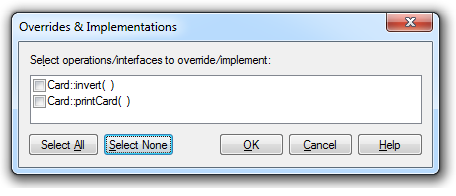
\includegraphics[width=0.6\textwidth]{ea_overrideDialogueModified}
  \caption{Selecting operations to override}  
  \label{ea:dialogue_override}
\end{center}
\end{figure}

\begin{figure}[htp]
\begin{center}
  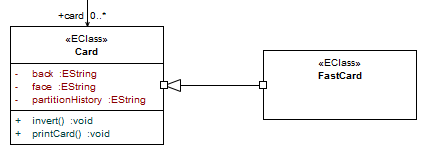
\includegraphics[width=0.9\textwidth]{ea_EClassFastCard}
  \caption{Fast cards are a special kind of card}  
  \label{ea:metamodel_FastCard}
\end{center}
\end{figure}

\vspace{0.5cm}

\item[$\blacktriangleright$] Now return to the \texttt{check} SDM (in \texttt{Partition}) and extend the control flow as depicted in
Fig.~\ref{ea:extendCheck}.

 \vspace{0.5cm}
 
\begin{figure}[htbp]
\begin{center}
  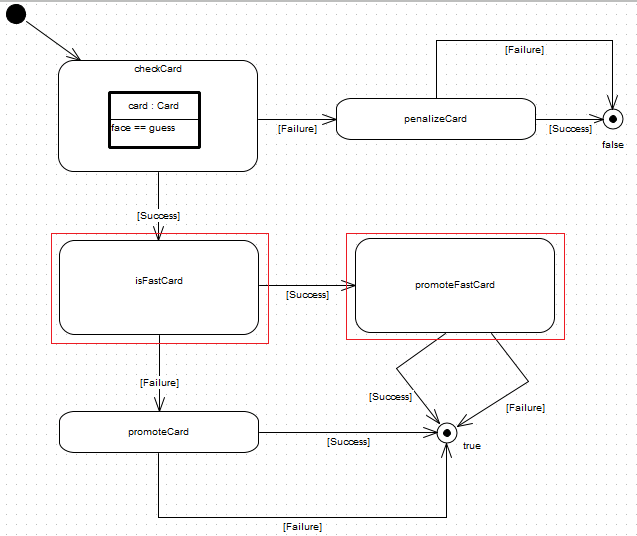
\includegraphics[width=\textwidth]{ea_extendCheck}
  \caption{Extend check to handle fast cards.}  
  \label{ea:extendCheck}
\end{center}
\end{figure}
 

\item[$\blacktriangleright$] As you can see, you have created two new story nodes, \texttt{isFastCard}, and \texttt{promoteFastCard}.
 
\item[$\blacktriangleright$] Next, in order to complete the newest conditional, create a bound \texttt{FastCard} object variable, named \texttt{fastcard} in
\texttt{isFastCard} (Fig.~\ref{ea:fastCardBinding}).
 
\item[$\blacktriangleright$] To check the dynamic type, we'll need to create a binding of \texttt{card} (of type \texttt{Card}) to \texttt{fastcard} (of
type \texttt{FastCard}), so edit the \texttt{Binding} tab in the \texttt{Object Variable Properties} dialogue (Fig.~\ref{ea:fastCardBinding}). Please note that
this tab will not allow any changes unless the \texttt{bound} option in \texttt{Object Properties} is selected. As you can see, this set up configures the
pattern matcher to check for types, rather than \texttt{parameters} and \texttt{attributes} as we've previously encountered.

\vspace{0.5cm}

\begin{figure}[htbp]
\begin{center}
  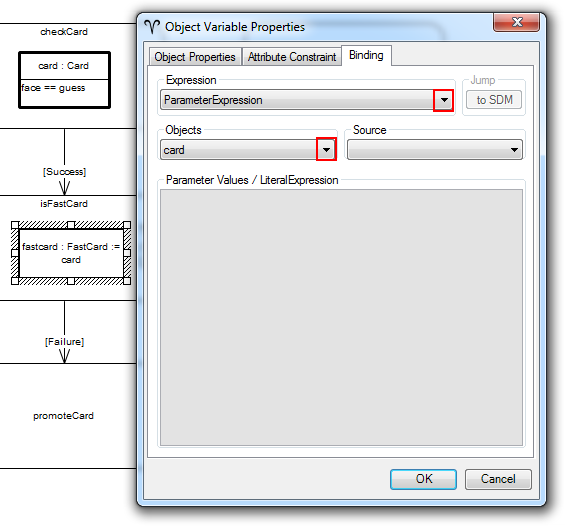
\includegraphics[width=0.9\textwidth]{ea_fastCardBinding}
  \caption{Create a binding for \texttt{fastcard}}  
  \label{ea:fastCardBinding}
\end{center}
\end{figure}

\clearpage

In our case, we could use a \emph{ParameterExpression} or an \emph{ObjectVariableExpression}\define{ObjectVariable\-Expression} as \texttt{card} is indeed a
parameter \emph{and} has already been used in \texttt{checkIfGuessIsCorrect}. We haven't tried the latter yet, so let's use \emph{ObjectVariableExpression}.

\item[$\blacktriangleright$] Update the \texttt{fastcard} binding by switching the expression to 
\texttt{Object\-Vari\-able\-Ex\-pres\-sion}, with \texttt{card} as the target. Note that a binding could also use a \emph{MethodCallExpression} to invoke a
method whose return value would be the bound value. This is very useful as it allows invoking helper methods directly in patterns.

\item[$\blacktriangleright$] To finalize the SDM, (i) extract the \texttt{promoteFastCard} story pattern and build the pattern according to
Fig.~\ref{ea:promoteFastCardPattern} and (ii) create the parallel \texttt{Success} and \texttt{Failure} edges from this activity to the stop node returning 
\texttt{true} for the same reason as in \texttt{check} earlier. Compare the pattern in Fig.~\ref{ea:promoteFastCardPattern} to Figs.~\ref{ea:sdm_check_complete_activity_node} and \ref{ea:sdm_check_complete_penalize}, the
original promotion and penalizing card movements. As you can see, they're very similar, except \texttt{fastCard} is transferred from the current partition
(\texttt{this}) immediately to the last partition in \texttt{box}, identified as having no next \texttt{Partition} with an appropriate NAC.
Note that a second NAC is used to handle the case where \texttt{this} would be the next \texttt{Partition}, which is also not what we want.

\begin{figure}[htbp] 
\begin{center}
  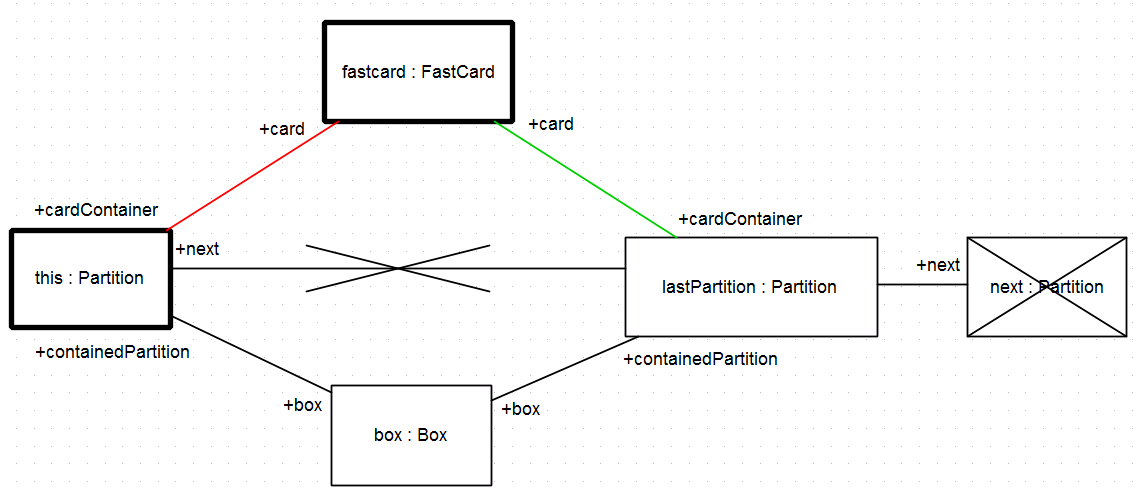
\includegraphics[width=\textwidth]{ea_promoteFastCardPattern}
  \caption{Story pattern for handling fast cards.}  
  \label{ea:promoteFastCardPattern}
\end{center}
\end{figure}

\item[$\blacktriangleright$] Inspect Fig.~\ref{eclipse:promoFastCardFinal} to see how this is done in the textual syntax.

\item[$\blacktriangleright$] You have now implemented every method using SDMs -- fantastic work! Save, validate, and build your metamodel to see some new code.
Inspect the implementation for \texttt{check}.  Can you find the generated type casts for \texttt{fastcard}?

\item[$\blacktriangleright$] At this point, we encourage you to read each of the textual SDM instructions to try and understand the full scope of eMoflon's
features (which start on page~\hyperlink{page.9}{9}) but you are of course, free to carry on.

\jumpSingle{subsec:fastGUI}

\end{itemize}
